\chapter{Analyse des principaux sites web}
\section{Objectif de l'analyse}
Le but de l'analyse est de parcourir les sites les plus visités au monde d'après le classement Alexa \cite{AlexaTop}. Ensuite, déterminer s'ils contiennent des trackers et, le cas échéant, leur nature. Deux types d'expérience peuvent être menés :
\begin{enumerate}
	\item Le premier consiste en une analyse à long terme.
	\item Le second consiste en une analyse ponctuelle.
\end{enumerate}

Le premier type d'expérience a pour but de déterminer si les sites modifient leurs trackers au fil du temps.
Le second type permet d'avoir une image globale du niveau de traçage opéré par les principaux sites à un instant donné. Il donne également la possibilité de tester l'efficacité des extensions de navigateur qui affirment protéger la vie privée (voir \autoref{results_plugins}).

\section{Description de l'outil implémenté}
L'idée initiale était d'utiliser le framework \textit{fpdetective} \cite{Acar:2013:FDW:2508859.2516674}. C'est un framework conçu pour la détection et l'analyse d'outils (\textit{fingerprinters}, voir \autoref{fingerprinters}) qui créent des empreintes de navigateurs. Ce framework semblait prometteur mais son efficacité s'est révélée insuffisante et il ne fonctionnait pas correctement. En effet, aucun \textit{fingerprinter} n'était détecté alors que certains étaient manifestement présents sur plusieurs sites web visités.

Etant donné que \textit{fpdetective} ne pouvait fournir les résultats demandés, la création d'un outil dédié à cette tâche était nécessaire. De plus, cela permettait davantage de souplesse au niveau des décisions d'implémentation et du paramétrage de la recherche de trackers.
\newline

L'outil a été implémenté en Java. Il se compose de deux éléments : le \textit{crawler} qui visite les sites web et exporte leur contenu au format HTTP Archive (HAR) et le \textit{parser} qui traite les fichiers HAR en déterminant si les sites correspondants renferment des trackers.
L'outil a été développé sous Eclipse et est destiné à être utilisé sur Linux. Un exécutable Jar est également disponible.
\newline

Lors du lancement du \textit{crawler}, l'utilisateur peut spécifier plusieurs arguments :
\begin{itemize}
	\item Requis : le mode (\textit{crawler} ou \textit{parser}).
	\item Requis : le répertoire des fichiers.\\
		Pour le \textit{crawler}, il s'agit du répertoire où les fichiers seront enregistrés.\\
		Pour le \textit{parser}, il s'agit du répertoire contenant les fichiers à analyser.
	\item Optionnel : l'activation du mode \textit{debug} qui va donner davantage de détails en cas de problème.
	\item Optionnel : l'affichage de l'aide.
	\newline
	\item Requis pour le \textit{crawler} : le profil de Firefox à utiliser.
	\item Requis pour le \textit{crawler} : le fichier contenant la liste des sites web à visiter.
	\item Requis pour le \textit{crawler} : le début de l'intervalle des sites à visiter.
	\item Requis pour le \textit{crawler} : la fin de l'intervalle des sites à visiter.
	\item Requis pour le \textit{crawler} : le nombre maximal de tentatives par site web (\textit{timeout}).
	\item Requis pour le \textit{crawler} : le nombre de sites à visiter avant le redémarrage de Firefox.
	\newline
	\item Requis pour le \textit{parser} : le fichier contenant la liste des trackers de Ghostery.
	\item Optionnel pour le \textit{parser} : l'activation de l'impression de tous les trackers identifiés.
\end{itemize}

\subsection{Crawler}
\label{crawler}
\subsubsection{Choix d'implémentation}
Afin d'automatiser le navigateur et de parcourir les sites sans intervention humaine, \textit{Selenium} \cite{selenium_homepage} est utilisé. Plus précisément, c'est le pilote \textit{FirefoxDriver} de \textit{Selenium} qui est utilisé au sein de l'outil.

La première implémentation traitait directement le code source de la page. Il était possible d'aller sur le moteur de recherche Google, de sélectionner le champ de recherche, de taper une requête et de récupérer le résultat. Cependant, le processus était assez lent et incomplet car on ne pouvait pas récupérer les requêtes et les réponses HTTP. On pouvait juste récupérer les éléments associés à des balises (par exemple, récupérer toutes les images via les balises de type \textit{<img>}, les scripts avec les balises \textit{<script>},...) mais tout n'était pas récupérable car certains éléments étaient chargés sans être identifiés.

Afin de pallier ce problème, la deuxième implémentation utilisait un proxy qui exportait le contenu du site au format HTTP Archive. L'ensemble des requêtes et réponses HTTP était récupéré et enregistré dans un fichier. Le parcours du code source (qui donnait des résultats finalement incomplets) a été supprimé afin de rendre le programme plus rapide. Cette fois, le problème était que le proxy n'exécutait pas le JavaScript. Il en résultait que de nombreux sites ne pouvaient être chargés correctement (cela pouvait varier de 15 à 30\% d'échecs) et il était alors impossible de les traiter.

La troisième solution, qui est la dernière implémentée, consiste à utiliser le pilote pour charger les sites automatiquement, sans parcours du code source ni utilisation de proxy. Le contenu des sites est exporté au format HTTP Archive à l'aide de deux extensions qui ont été installées dans Firefox.
\begin{itemize}
	\item La première, Firebug \cite{firebug_homepage}, est une extension utilisée principalement par les développeurs de sites web afin de les débugger. Elle permet de monitorer les éléments d'une page (CSS, HTML, JavaScript) en direct.
	\item La seconde, NetExport \cite{netexport_homepage}, est une extension de Firebug qui permet d'exporter toutes les données d'une page au format HTTP Archive de façon automatique (il est possible de paramétrer cette extension pour le faire).
\end{itemize}

Le taux de réussite de l'export des données des sites s'est grandement amélioré. Néanmoins, certains sites ne sont toujours pas chargés correctement.
Une hypothèse est que certains sites sont hébergés sur des serveurs lointains et leurs éléments prennent alors plus de temps à charger. Ainsi, lorsque ces sites contiennent une grande quantité d'éléments, le pilote renvoie une exception de type \textit{timeout} et le chargement du site est finalement en échec. On remarque généralement ceci sur les sites asiatiques : certains portails regorgent de contenus qui prennent du temps à charger.
Une hypothèse supplémentaire est que certains sites demandent une action de l'utilisateur (faire défiler la page par exemple) afin de charger les éléments du site (typiquement, les images).
\newline

Une amélioration a été apportée à l'outil afin de compter le nombre de cookies Flash et de cookies classiques (qu'ils soient enregistrés via les réponses HTTP ou des scripts JavaScript) lors de chaque visite de site. Cette fonctionnalité a été implémentée au sein du \textit{crawler} étant donné que ce n'est pas possible d'accéder à cette information avec l'aide des fichiers HTTP Archive analysés par le \textit{parser}. Cela signifie qu'une partie des résultats est déjà disponible lorsque le \textit{crawler} a fini de visiter les sites.

A son lancement, il supprime l'ensemble des cookies Flash (les fichiers .sol) dans le dossier \textit{.macromedia/Flash\_Player/\#SharedObjects/XXXXXXXX/}. Il supprime également les cookies Firefox en se connectant à la base de données SQLite dans \textit{.mozilla/firefox/<profil>/cookies.sqlite} et en vidant la table \textit{moz\_cookies}. Cela permet de s'assurer que la visite des sites ne sera pas influencée par la présence de cookies antérieurs.

\subsubsection{Changements opérés sur les extensions}
\label{changements_extensions}
Deux modifications ont été nécessaires sur l'extension \textit{NetExport} de \textit{Firebug}.

La première concerne la génération des fichiers HTTP Archive. Par défaut, l'extension ajoute un champ qui n'est pas standard par rapport à la spécification du format HAR. Il en résulte que les fichiers peuvent alors être considérés comme corrompus alors que la présence ou non de ce champ n'influence en rien les résultats qui nous concernent. La génération de ce champ a donc été supprimée dans le fichier \textit{/chrome/content/netexport/harBuilder.js} de \textit{NetExport}.

La seconde modification concerne le nom des fichiers générés. Par défaut, l'extension ajoute la date à l'URL du site dans les noms de fichier. Cela pose des difficultés supplémentaires au \textit{parser} lors de la récupération et du traitement de ces fichiers (voir \autoref{parser}). L'extension a donc été modifiée afin de n'utiliser que l'URL du site dans les noms du fichier. Cette modification a été effectuée dans le fichier \textit{/chrome/content/netexport/automation.js}. Sur Linux, lorsqu'un fichier de même nom existe déjà, un tiret suivi du numéro de copie est ajouté au nom de fichier avant son extension.

\subsubsection{Fonctionnement}
Le \textit{crawler} fonctionne de la manière suivante. D'abord, il vérifie que le répertoire donné en argument est accessible en écriture et il crée deux dossiers nommés "logs" et "results" qui sont destinés à contenir respectivement les logs et les résultats du \textit{crawler}. Ensuite, le fichier de log (log\_crawler.txt) est créé, le dossier des cookies Flash est détecté (s'il y en a plusieurs, l'utilisateur est invité à indiquer le bon dossier) et la base de données SQLite des cookies Firefox est vidée (le dossier des paramètres de l'utilisateur est automatiquement trouvé grâce au profil Firefox spécifié en argument au lancement du programme). La liste des sites à visiter est ainsi chargée depuis le fichier spécifié et en fonction de l'intervalle donné par l'utilisateur. Puis, le profil Firefox choisi est chargé et différents paramètres de configuration des extensions sont également réglés avant que le pilote ne soit initialisé et qu'il lance Firefox. Après le lancement du pilote, un délai de 5 secondes laisse le temps à Firefox de se lancer et de charger ses extensions.
\newline

Après cette phase de préparation, le parcours des sites commence. Le pilote dirige Firefox sur l'URL du premier site de la liste. Lorsque le chargement de la page est terminé, un délai de 8 secondes permet aux extensions d'enregistrer le fichier HTTP Archive. Le nombre de cookies Flash est enregistré pour chaque site.

Si la page s'est chargée avant la limite de 30 secondes, l'enregistrement est considéré comme valide et le pilote charge le site suivant dans la liste.

Si un site fait un timeout et que l'utilisateur a précisé un nombre de tentatives supérieur à 1, le pilote dirige Firefox sur la page "about:blank" (cela permet d'éviter des problèmes d'écriture de fichiers avec les extensions) puis le redirige sur le site pour un nouvel essai. Ce processus est répété à chaque timeout jusqu'à atteindre le nombre maximal de tentatives. Si le site fait encore un timeout lors de la dernière tentative, il est alors considéré en échec et son URL est inscrite dans une liste reprenant tous les sites en échec. A la deuxième tentative, l'URL du site a déjà été enregistrée dans une autre liste reprenant tous les sites ayant fait un timeout, cela permet de garder une trace des sites dont la visite a rencontré un problème mais qui ont finalement pu être chargés. 

Il arrive également qu'un site ne puisse tout simplement pas être chargé (à cause d'une erreur dans son code source par exemple). Son URL est alors directement enregistrée dans la liste reprenant les sites en échec.
\newline

Lorsque le parcours de l'ensemble des sites est terminé, le programme efface les fichiers inutiles générés lors de la visite des pages "about:blank" et détaille l'ensemble des sites ayant subi au moins un timeout et les sites en échec. La liste des sites avec leur nombre de cookies Flash est enregistrée en ordre décroissant dans le fichier "stats\_flash-cookies.csv" du dossier "results". Pour terminer, le pilote est arrêté (ce qui entraîne la fermeture de Firefox) et le fichier de log est fermé.
\newline

Il a été nécessaire d'implémenter une fonctionnalité qui redémarre Firefox à intervalles réguliers. En effet, certains sites ouvrent des pop-ups et si le navigateur n'est pas fermé, ces derniers s'accumulent et occupent une part plus importante de ressources. Le redémarrage du navigateur permet de fermer toutes ces fenêtres ouvertes de façon intempestive afin de garantir une meilleure stabilité du \textit{crawler}.

\subsection{Parser}
\label{parser}
\subsubsection{Choix d'implémentation}
Lors de la visite des sites par le \textit{crawler}, il arrive que celui-ci doive refaire de nouvelles visites afin d'exporter correctement le fichier HTTP Archive d'un site. Il en résulte que plusieurs fichiers pour le même site soient disponibles. Par exemple, on peut très bien voir des fichiers tels que \textit{monsite.com.har}, \textit{monsite.com-1.har}, etc. Lors de l'analyse de ces fichiers par le \textit{parser}, celui-ci considère seulement la dernière version du fichier comme étant valide. Il ignore donc les autres fichiers concernant le même site (si jamais il y en a plusieurs) car ils sont généralement corrompus ou incomplets.
\newline

Lors de l'analyse d'un site, l'autorité en charge pour son domaine est automatiquement récupérée via une requête DNS de type SOA. Cela permet de déterminer si une URL présente dans le site appartient au même domaine ou si elle provient d'un domaine différent.

Si l'autorité du site analysé ne peut être récupérée, l'analyse du site est considérée comme étant en échec et le nom du fichier contenant les informations de ce site est ajouté dans une liste reprenant tous les fichiers en échec.

Si l'autorité du domaine d'une URL ne peut être récupérée, l'analyse de cette URL est passée mais l'analyse des URL suivantes du fichier continue. Un message est imprimé dans le log pour préciser que la récupération de l'autorité du domaine d'une URL a subi un problème.

Lorsqu'une URL est constituée d'une adresse IP, l'outil fait une requête DNS afin de connaître le nom associé à cette IP. S'il n'y parvient pas, l'analyse de l'URL est passée mais le processus d'analyse continue comme c'est le cas lorsqu'une autorité ne peut être récupérée pour une URL. Ceci est dû au fait que la libraire utilisée (\textit{dnsjava}) n'est pas en mesure d'effectuer des requêtes SOA pour des adresses IP.

Le fonctionnement de la récupération de l'autorité d'une URL est le suivant : tout d'abord, la requête est effectuée sur l'hôte de l'URL. Si aucune réponse n'est retournée, la requête est effectuée sur le domaine parent et ainsi de suite, jusqu'à trouver une réponse ou arriver au domaine le plus haut.

Un système de mise en cache a été mis en place afin de limiter le nombre de requêtes effectuées et d'améliorer la rapidité d'accès à l'information.

\subsubsection{Limitation des requêtes DNS de type SOA}
Le recours aux informations SOA permet généralement de déterminer si deux sites appartiennent au même domaine. C'est ainsi que lors de la visite de \textit{youtube.com}, les images provenant de \textit{ytimg.com} ne sont pas détectés comme provenant d'un site externe (voir \autoref{dig_youtube} et \autoref{dig_ytimg}).

\begin{figure}[h]
	\centering
	\lstinputlisting[style=dig]{examples/dig_youtube.com}
	\caption{\label{dig_youtube}Informations SOA pour \textit{youtube.com}}.
\end{figure}

\begin{figure}[h]
	\centering
	\lstinputlisting[style=dig]{examples/dig_ytimg.com}
	\caption{\label{dig_ytimg}Informations SOA pour \textit{ytimg.com}}.
\end{figure}
Comme vous pouvez le voir, les sites \textit{youtube.com} et \textit{ytimg.com} sont sous la même autorité qui est \textit{dns-admin@google.com}. Dans ce cas, toute URL présente dans le site \textit{youtube.com} provenant de \textit{ytimg.com} ne sera pas considérée comme extérieure au site.
\newline

Cependant, il peut y avoir des faux positifs résultant des réponses reçues. C'est ainsi que lors des analyses, un phénomène a été remarqué: à certains moments, la requête DNS peut renvoyer une réponse différente. Ceci a été remarqué pour le site \textit{p8.qhimg.com} (voir \autoref{dig_p8.qhimg.com_1} et \autoref{dig_p8.qhimg.com_2}). Dans ce précis, la requête DNS précise que l'autorité du site est en fait celle de l'hébergeur de contenu \textit{cloudfront.net} (qui est lui-même hébergé sur les serveurs d'\textit{Amazon}) et non plus celle du site visité. Cela dépend en fait de l'infrastructure de leur hébergement et ceci ne pourrait être pris en compte au sein de l'outil sans ralentir de façon conséquente ses performances.

\begin{figure}[h]
	\centering
	\lstinputlisting[style=dig]{examples/dig_p8.qhimg.com_1}
	\caption{\label{dig_p8.qhimg.com_1}Informations SOA pour \textit{p8.qhimg.com}}.
\end{figure}

\begin{figure}[h]
	\centering
	\lstinputlisting[style=dig]{examples/dig_p8.qhimg.com_2}
	\caption{\label{dig_p8.qhimg.com_2}Informations SOA pour \textit{p8.qhimg.com}, 10 secondes plus tard}.
\end{figure}

\subsubsection{Critères qualifiant un tracker}
Le \textit{parser} parcourt l'ensemble des requêtes et réponses HTTP effectuées lors du chargement du site. Afin de déterminer si une ressource chargée est un tracker, l'outil se base sur plusieurs critères.
\begin{itemize}
  \renewcommand{\labelitemi}{$\Rightarrow$}
 \item Présence de l'URL dans la base de données de trackers Ghostery
 \item Si l'URL n'est pas présente dans la base de données Ghostery, l'autorité du domaine de l'URL est récupérée et comparée à celle du site visité.\\
		Si les autorités sont différentes, les critères suivants permettent de déterminer si l'URL est un tracker:
		\begin{itemize}
			\item Un cookie est créé via la réponse HTTP
			\item La ressource chargée est du JavaScript
			\item La ressource chargée est du Flash
			\item Les images chargées ont une largeur et hauteur de 1 pixel (pixels espions)
			\item L'URL des ressources chargées contient des paramètres
			\newline
		\end{itemize}
\end{itemize}

Afin de pouvoir utiliser la base de données Ghostery \cite{ghostery_homepage}, un contact a été pris avec Evidon (les développeurs de l'extension) qui a donné son autorisation d'utiliser la base de données au sein de cet outil.
\newline

Il est évident que certains de ces critères peuvent mener à des faux positifs mais potentiellement chaque ressource chargée d'un site externe permet de tracer l'utilisateur. Dans ses logs, l'administrateur d'un site peut déterminer à quelle heure et quelle ressource un utilisateur a demandé (cela est particulièrement utilisé par les pixels espions).

Au-delà de cette première donnée, l'administrateur du site peut également enregistrer un cookie sur l'ordinateur de l'utilisateur afin de l'identifier s'il recharge une ressource du serveur ultérieurement.

Le fichier JavaScript provenant d'un site externe peut également créer des cookies sans l'autorisation du site qui fait appel à ce script.

Le chargement de ressources contenant des paramètres repose sur le même principe que l'analyse des logs sauf qu'il permet d'aller plus loin en précisant un identifiant pour chaque site qui souhaite charger des ressources d'un autre site.

\subsubsection{Fonctionnement}
Le but du \textit{parser} est de traiter les fichiers HTTP Archive générés par le \textit{crawler} et de déterminer le nombre de trackers pour chaque site. La première chose qu'il fait à son lancement est de vérifier que le dossier donné en argument est accessible en écriture. Il regarde ensuite si des dossiers "logs" ou "results" sont déjà présents et si ce n'est pas le cas, il les crée. S'ils sont déjà présents, le \textit{parser} avertit l'utilisateur qu'il va les utiliser afin d'y écrire des données. Concernant le dossier "results", il demande à l'utilisateur s'il souhaite continuer car des fichiers provenant de résultats calculés antérieurement pourraient être écrasés. Puis, le \textit{parser} ouvre un fichier de log ("log\_parser.txt" dans le sous-dossier "logs"). Ensuite, il charge l'ensemble des sites comme expliqué ci-dessus, il ouvre le fichier contenant la base de données de trackers Ghostery et charge l'ensemble des expressions régulières utilisées afin de détecter les trackers. L'analyse des fichiers HTTP Archive commence et exporte pour chaque site analysé de multiples informations telles qu'expliqué dans la sous-section précédente. Lorsque tous les fichiers ont été analysés, le \textit{parser} calcule les statistiques pour l'ensemble de l'analyse. Ensuite, il indique le nombre de fichiers ayant été correctement analysés et détaille les fichiers n'ayant pu être traités. Pour terminer, il ferme le fichier de log.

\subsection{Format des résultats}
Il existe deux types de résultats : les résultats détaillés pour chaque fichier HTTP Archive analysé et les résultats globaux de l'analyse.

Les résultats globaux sont enregistrés dans le dossier "logs" alors que les résultats détaillés sont enregistrés dans le dossier "results".
Ceci a été décidé par souci de simplicité car les résultats globaux sont ainsi directement accessibles et ne sont pas noyés dans le dossier contenant les résultats détaillés.

\subsubsection{Crawler}
Les résultats globaux dans le dossier "logs" :
\begin{itemize}
	\item \textbf{stats\_flash-cookies.csv} contient la liste des sites utilisant des cookies Flash, triés par ordre décroissant.
	%\newline
\end{itemize}

\subsubsection{Parser}
Les résultats globaux dans le dossier "logs" :
\begin{itemize}
	\item \textbf{stats\_mimetypes.csv} contient la liste des types d'éléments (\textit{mimetype}) chargés d'un domaine différent, triés par ordre décroissant.
	\item \textbf{stats\_detailed.csv} contient la liste des sites avec le nombre détaillé de trackers (trackers connus identifiés avec l'aide de Ghostery, réponses HTTP créant un cookie, fichiers JavaScript et Flash chargés depuis un autre domaine, pixels espions et requêtes effectuées avec des paramètres).
	\item \textbf{stats\_trackers.csv} contient la liste des trackers identifiés grâce à Ghostery, triés par ordre décroissant.
	\item \textbf{stats\_websites.csv} contient la liste des sites avec le nombre de trackers identifiés, triés par ordre décroissant.
	\newline
\end{itemize}

Les résultats détaillés pour chaque site dans le dossier "results" :
\begin{itemize}
	\item \textbf{<URL du site>\_cookies.csv} contient la liste des cookies créés par des réponses HTTP d'un domaine différent.
	\item \textbf{<URL du site>\_flash.csv} contient la liste des fichiers Flash provenant d'un autre domaine.
	\item \textbf{<URL du site>\_js.csv} contient la liste des fichiers JavaScript provenant d'un domaine tiers.
	\item \textbf{<URL du site>\_mimetypes.csv} contient la liste des types d'éléments (\textit{mimetype}) chargés d'un domaine différent, triés par ordre décroissant.
	\item \textbf{<URL du site>\_parameters.csv} contient la liste des requêtes vers un domaine différent dont l'URL contient des paramètres.
	\item \textbf{<URL du site>\_pixels.csv} contient la liste des pixels espions détectés depuis un autre domaine.
	\item \textbf{<URL du site>\_urls.csv} contient la liste de l'URL de toutes les ressources chargées d'un domaine différent.
	\newline
\end{itemize}

\section{Résultats}

\subsection{Expérience 1 : étude à long terme}
\subsubsection{Détails de l'expérience}
Le but de cette expérience est de déterminer l'évolution des trackers sur une certaine période en effectuant des mesures de façon régulière.

Afin de réaliser cette étude, le \textit{crawler} a été lancé chaque jour du 28 mars au 7 mai 2014 (à l'exception du 8 avril) sur le TOP 1000 du classement Alexa \cite{AlexaTop}, ce qui représente 40 jours de mesures. Notez cependant que l'implémentation du compteur de cookies Flash a été réalisée ultérieurement à cette expérience et ces données ne sont donc pas disponibles au sein de l'expérience.
\newline

Le \textit{crawler} a été lancé avec les paramètres suivants :
\begin{itemize}
	\item les sites visités sont issus du TOP Alexa du 26 mars 2014
	\item l'intervalle sélectionné concerne les 1000 premiers sites
	\item 3 tentatives maximum ont été autorisées par site
	\item Firefox était redémarré tous les 50 sites
	\item Firefox était dépourvu de toute extension (autre que Firebug et NetExport)
	\newline
\end{itemize}

\subsubsection{Premières constatations}
Lors de cette expérience, on peut voir que le taux d'échec avec le \textit{crawler} est toujours inférieur à 9\%.
Notez que l'implémentation a un peu changé depuis cette expérience. Lors de cette dernière, quand un site atteignait le nombre maximum de tentatives et qu'il était placé dans la liste des sites en échec, il était également retiré de la liste des sites ayant eu besoin d'au moins un nouvel essai suite à un timeout.
Ceci explique des situations telles que sur la \autoref{Exp1_crawler_fails} au début du mois de mai.

\begin{figure}[h]
	\centering
	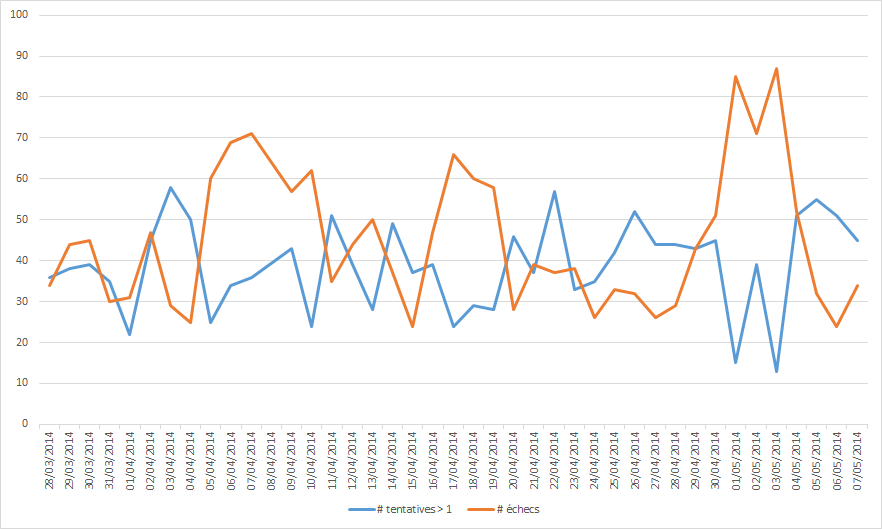
\includegraphics[scale=.7]{graphiques/Exp1_crawler_fails.png}
	\caption{\label{Exp1_crawler_fails}Le nombre d'échecs du \textit{crawler}}.
\end{figure}

\begin{figure}[h]
	\centering
	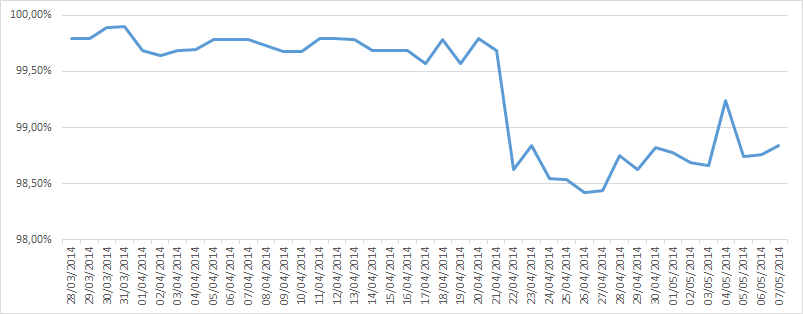
\includegraphics[scale=.8]{graphiques/Exp1_parser_success_rate.png}
	\caption{\label{Exp1_parser_success_rate}Le pourcentage de réussite du \textit{parser}}.
\end{figure}

Le pourcentage de fichiers correctement analysés est représenté à la \autoref{Exp1_parser_success_rate}. On peut voir que du début de l'expérience jusqu'au 21 avril, le pourcentage de réussite est en moyenne de 99,73\%. A partir du 22 avril et jusqu'à la fin de l'expérience, il passe à 98,71\%. Cela représente une dizaine de fichiers.
Croyant d'abord à une erreur lors de l'exécution du \textit{parser}, les analyses ont été reconduites une seconde fois mais n'ont pas montré de résultat différent.
Après analyse des fichiers de log du \textit{parser}, on remarque que ce sont généralement les mêmes sites qui sont en échec.
Ainsi, sur les 16 jours (du 22 avril jusqu'au 7 mai), on peut remarquer certains faits.
\newline
Les sites suivants étaient chaque jour en échec:
\begin{itemize}
  \item 9gag.com
  \item mashable.com
  \item www.pixiv.net
  \item www.wikihow.com
  \newline
\end{itemize}
Les sites suivants n'ont pas été en échec 1 jour :
\begin{itemize}
  \item www.gamespot.com : le 4 mai
  \item www.theverge.com : le 4 mai
  \newline
\end{itemize}
Les sites suivants n'ont pas été en échec 2 jours :
\begin{itemize}
  \item www.thefreedictionary.com : le 25 avril et le 4 mai
  \item www.wix.com : le 28 avril et le 4 mai
  \newline
\end{itemize}
Les sites suivants ont été en échec sur une période de plusieurs jours :
\begin{itemize}
  \item www.rednet.cn : 3 jours (du 25 au 27 avril)
  \item chinaz.com : 2 jours (les 27 et 28 avril)
  \item www.groupon.com : 2 jours (les 5 et 6 mai)
  \newline
\end{itemize}
Les sites suivants n'ont été en échec qu'un seul jour :
\begin{itemize}
  \item www.suning.com : le 22 avril
  \item baomihua.com : le 24 avril
  \item bleacherreport.com : le 26 avril
  \item www.aili.com : le 27 avril
  \item www.hm.com : le 30 avril
  \item www.businessinsider.com : le 3 mai
  \newline
\end{itemize}
Les autres sites en échec ne peuvent pas être classés de manière identique.\\

La constatation que certains sites sont en échec pendant la période complète des 16 jours (alors qu'ils ne l'étaient pas avant le 22 avril) et que certains sites sont en échec sur une courte période (2-3 jours) fait penser que ces échecs résultent d'une erreur située sur les sites eux-mêmes.
\newline

Une recherche approfondie a été effectuée et celle-ci a confirmé l'hypothèse selon laquelle l'erreur provient des données reçues des serveurs. Plus précisément, les erreurs proviennent de champs non reconnus dans les réponses HTTP ou de valeurs erronées. Quelques exemples illustrant les erreurs rencontrées ont été ajoutés.
\newline

\begin{figure}[h]
	\centering
	\lstinputlisting[style=dig]{examples/bad_field_google}
	\caption{\label{bad_field_google}Réponse HTTP de \textit{Google} qui veut créer un cookie avec un champ "priority"}.
\end{figure}

\begin{figure}[h]
	\centering
	\lstinputlisting[style=dig]{examples/bad_field_baidu}
	\caption{\label{bad_field_baidu}Réponse HTTP de \textit{Baidu} avec un champ "domian" au lieu de "domain"}.
\end{figure}

\begin{figure}[h]
	\centering
	\lstinputlisting[style=dig]{examples/bad_field_gamespot}
	\caption{\label{bad_field_gamespot}Réponse HTTP de \textit{GameSpot} avec la valeur "0" pour le champ "expire"}.
\end{figure}

\subsubsection{Nombre de trackers}
Le nombre total de trackers semble rester stable, il est en moyenne de 30080. Ce nombre chute le 2 avril où il est de 25770 trackers. Ceci s'explique par le fait que le nombre de fichiers HTTP Archive pour ce jour (845 fichiers) est inférieur comparé aux autres jours, ce qui fait que moins de sites ont pu être analysés. Le nombre inférieur de fichiers provient probablement d'une perte de données suite à une suppression accidentelle ou à un manque d'espace disque qui a empêché l'enregistrement des fichiers HTTP Archive.

\begin{figure}[h]
	\centering
	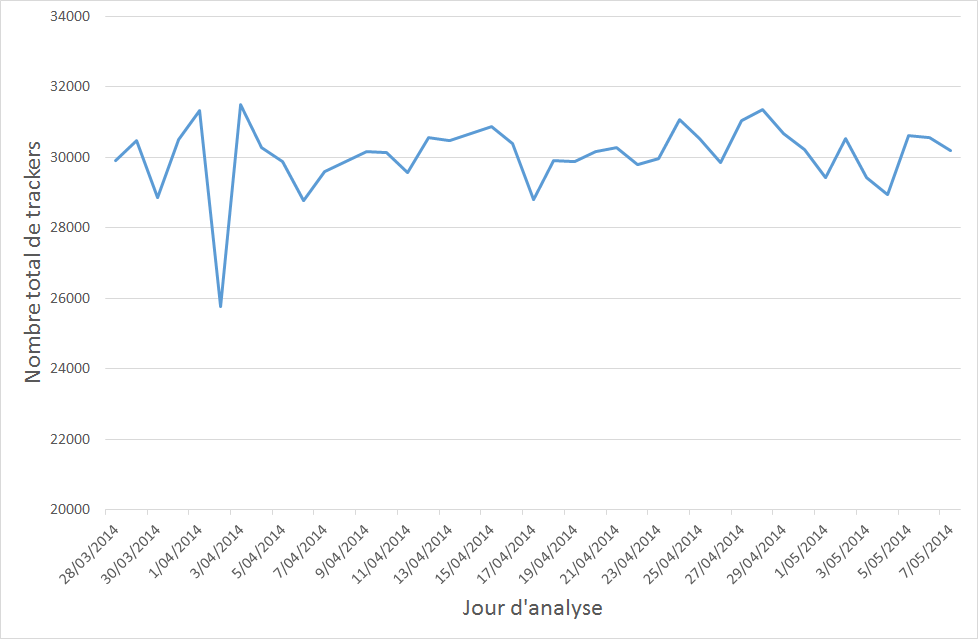
\includegraphics[scale=.8]{graphiques/Exp1_parser_total_trackers.png}
	\caption{\label{Exp1_parser_total_trackers}Nombre total de trackers sur l'ensemble de l'analyse}.
\end{figure}
\subsection{Expérience 2 : étude ponctuelle}

\subsubsection{Sites renfermant le plus de trackers détectés}

\subsubsection{Organisations déployant le plus de trackers}
